\documentclass[12pt]{article}
\usepackage{amsmath}
\usepackage[margin = 1in]{geometry}
\usepackage{graphicx}
\usepackage{booktabs}
\usepackage{natbib}
\usepackage{url}
\usepackage[colorlinks=true, citecolor=blue]{hyperref}

%% meta data
\title{Data analytics effects in Baseball player's value}
\author{Chenyu Mu\\
  Department of Statistics\\
  University of Connecticut
}

\begin{document}

\maketitle

\begin{abstract}
  Over the past two decades, there has been a notable resurgence in the utilization of data analytics across 
  professional sports, businesses, and governmental sectors. We can measure the value of baseball players through
  data analysis, which is very important to the success of the team. Therefore, this article will study how to 
  measure the value of a player and will delve into an in-depth analysis of the myriad factors that potentially 
  impact baseball players while they are actively engaged in the game. 
\end{abstract}


\section{Introduction}
\label{sec:intro}
  
The surge in the availability of data, from player statistics to in-game metrics, has ushered in a new era in 
baseball analysis. This wealth of information has not only enriched the fan experience but has also become an 
invaluable tool for teams and analysts seeking a competitive edge. So how do we measure the value of players in
a statistical way?Before discussing how to measure value, we need to discuss the definition of value. 
According to the definition in Wyers' article "How to measure a player's value"\cite*{web:Wyers:Part1}, we define 
the value of a player as "A player's value is his contributions to his team based upon his on-field performance 
(hitting, running, fielding and pitching) in a neutral context.This definition excludes qualities like leadership 
and character, which would be horrific to see a statistical measure of performance attempt to portray! That's not 
to argue these things don't matter; they just aren't easily quantified. In addition, according to Wyers' approach, 
we need to emphasize that this is a neutral environment. First, we want to quantify a player's performance apart 
from his teammates' - a player is no better or worse on a good or terrible team. Besides, we aim to separate a 
player from his surroundings. A terrible pitcher does not become a better pitcher by pitching in Petco Park, and 
a poor hitter does not become a better pitcher by hitting in Coors Field.\\

We should realize there are some limits may effects our statistical model:
\begin{enumerate}
\item The data itself. Errors can occur, including transcription errors and similar inaccuracies. Additionally, 
certain determinations rely on borderline judgments, such as discerning whether an event constitutes a hit or an
error, categorizing a hit as a fly ball or a line drive, and determining whether a pitch is a ball or a strike.

\item Critical information might be omitted from the data, necessitating inference or deliberate oversight. 
Questions such as the shortstop's positioning on the field or whether the coach executed a hit-and-run strategy may 
not be explicitly recorded and might require additional interpretation or intentional exclusion.

\item Developing a model without a grasp of the fundamental principles poses challenges. The inherent value
difference between a double and a sacrifice fly in baseball may be intuitive, but expressing and capturing this 
nuanced understanding can be particularly challenging for a linear regression model.

\item The model overlooks certain factors, such as the quality of the opponent, platoon advantage, and other 
relevant considerations.

\item Neglecting to consider subtle distinctions between players, such as the influence of a ballpark on the home 
run rates of individuals like Barry Bonds and Juan Pierre, can lead to oversights in the analysis.
\end{enumerate}




\cite*{web:Wyers:Part2}

% roadmap
The rest of the paper is organized as follows.

The data will be presented in Section~\ref{sec:data}.

The methods are described in Section~\ref{sec:meth}.

The results are reported in Section~\ref{sec:resu}.

\section{Data}
\label{sec:data}
Following are definitions we may use:\\
$AB$: At bats\\ 
$AVG$: Batting average\\ 
$H$: Hits\\
$K$: Killed,Strikeout \\
$HR$: Home Run\\
$BABIP$: Batting Average on Balls in Play\\
$SF$: sacrifice flies\\
\begin{equation}
  \label{eq:AVG}
  AVG = H/AB,
\end{equation}
which means the total number of hits divided by the total number of at-bats
\begin{equation}
  \label{eq:BABIP}
  BABIP = (H - HR) / (AB - K - HR - SF),
\end{equation}
which states that a batter's average for balls that are put in play (excludes strikeouts, home runs, and sacrifice flies)


We can see the number of players in each team in Figure~\ref{fig:team}.
\graphicspath{{images/}}

\begin{figure}[tbp]
  \centering
  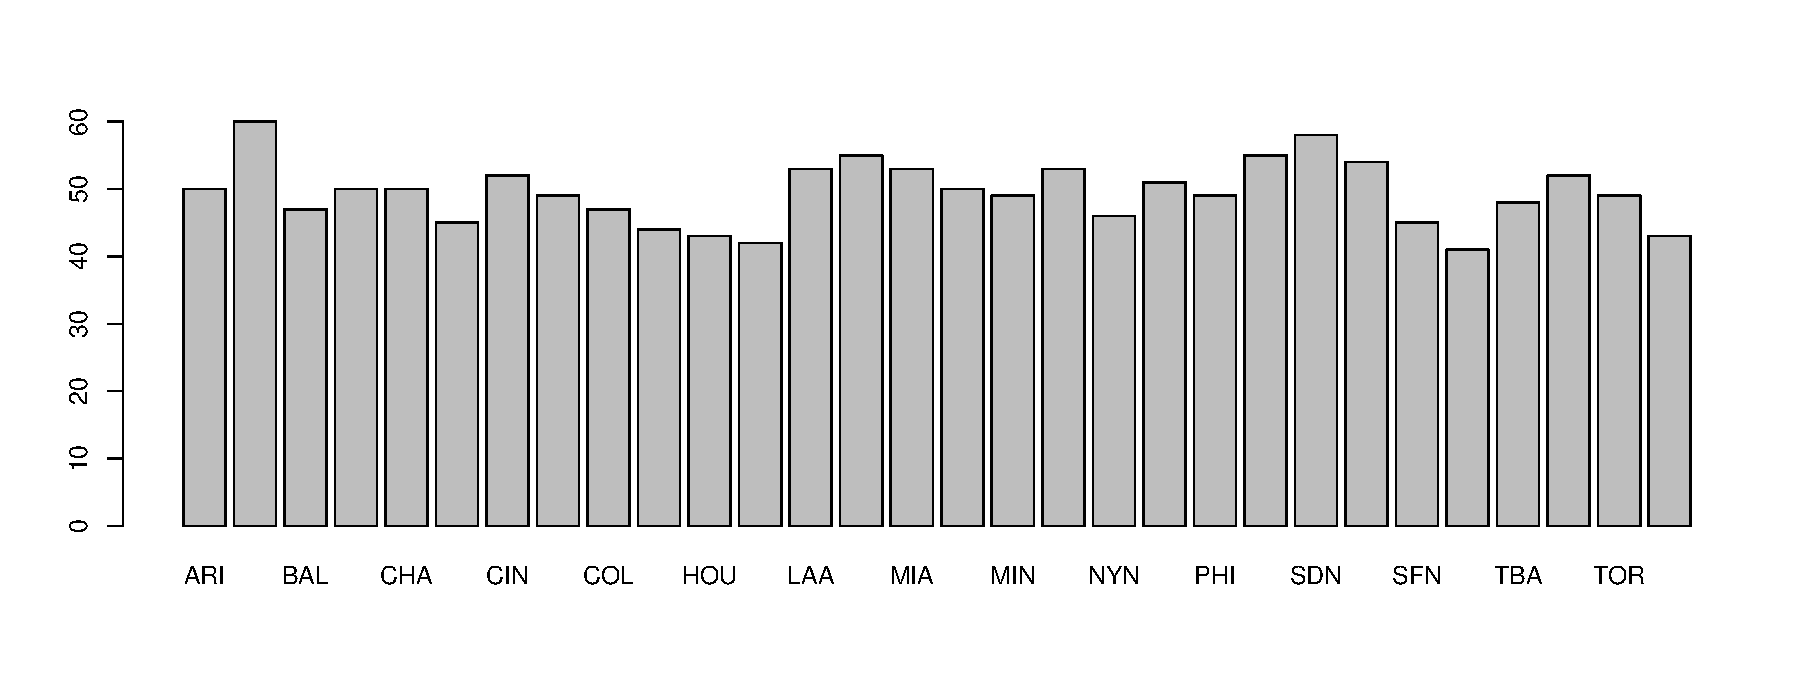
\includegraphics[width=\textwidth]{baseball team.pdf}
  \caption{The number of players in each team in 2016 batting dataset}
  \label{fig:team}
\end{figure}

\section{Methods}
\label{sec:meth}
We will use UConn baseball team data for our research and use Wyers's method \citet*{web:Wyers:Part2} that "
A player's value is essentially an average team's runs or wins with that player, minus their runs or wins without 
that player."



\section{Results}
\label{sec:resu}
These limitations encompassed various factors, including but not restricted to the sample size, the participants' in-season playing time,
and the number of at-bats and innings pitched. The relatively small sample size utilized in the study, which significantly impacted the practicality of the results Table~\ref{tab:rv}.

\begin{table}[tbp]
  \caption{The distribution of censored participants}
  \label{tab:rv}
\centering
\begin{tabular}{rrrr}
  \toprule
  Position & Assigned Group & Did Not Meet AB or IP & Did Not Play\\ 
  \midrule
Pitcher & Control & 3 & 1\\
Pitcher & Experiment & 2 & 1\\
Infield & Control & 1 & 0 \\
Infield & Experiment & 2 & 2\\
Outfield & Control & 1 & 0\\
Outfield & Experiment & 1 & 0\\
  \bottomrule
\end{tabular}
\end{table}

The study involved recruiting 26 members from the baseball team. Among these participants, 0.385, were pitchers, 0.423 were infielders, and 0.192 were outfielders. 
Splitting these groups, half of the pitchers were in the control group, while the remaining half were in the experimental group. For the infielders, 
0.455 were in the control group, and 0.545 were in the experimental group. As for the outfielders, 0.4 were in the control group, and 0.6 were in the experimental group.
Due to limitations in the sample size—considered small—the study's reliability may have been affected since it was conducted as a convenience sample. 
While the recruitment method was straightforward as it targeted the university's varsity team, the size of the sample could potentially impact the study's outcomes. 
Notably, the study would have ideally required a minimum sample size of 128, calculated using a specific formula considering an alpha level of .05, t-tests for independent groups, 
an effect size of 0.5, and a power of 0.8. Implementing this study on a larger scale, such as within a Minor League Baseball organization, 
would have made achieving the required sample size more feasible. 


\bibliographystyle{plain}
\bibliography{refs}

\end{document}